\documentclass[../lecture-notes-148x210.tex]{subfiles}


\begin{document}
\subsection*{Sum-Check Toolkit}

\subsection{Sum-Check-based Protocol for Grand Products}
\label{sec:grand-products}

This subsection describes a transparent SNARK, which may be used for proving grand product relations of the following form:
\begin{equation}
\mathcal{R}_{GP} = \big\{ (p \in \mathbb{F}, \mathbf{v} \in \mathbb{F}^m)\colon p = \prod_{i=0}^m v_i \big\} \label{grand-product-relation}
\end{equation}
Let $m = |\mathbf{v}|$. WLOG, assume that $m$ is a power of $2$.
We can think of $\mathbf{v}$ as a vector of evaluations of a $\log m$-variate multilinear polynomial $v(x)$ over 
$\{0, 1\}^{\log m}$ in a natural fashion. We assume the prover first opens $p$ and then commits to $v(x)$; the 
ensuing protocol then verifies both the polynomial’s validity and the corresponding grand-product equality derived
 from that commitment.

\begin{lemma}
A scalar $p$ and a vector $\mathbf{v}$ satisfies the relation $\mathcal{R}_{GP}$ if and only if there exists a 
multilinear polynomial $f$ in $\log m + 1$ variables such that $f(1,\dots,1, 0) = p$ and $\forall x \in \{0,1\}^{\log m}$
 the following hold:
\begin{gather*}
f(0, x) = v(x)\\
f(1,x) = f(x, 0) \cdot f(x, 1)
\end{gather*}
Such polynomial $f$ has the following construction: \begin{itemize}
    \item $f(1,\dots,1) = 0$
    \item For all $\ell \in [\log m]$ and $x \in \{0,1\}^{\log m - \ell}$: \\ 
    \vspace{-0.8em}
    \begin{equation*}
        f(1^\ell, 0, x) = \prod_{y \in \{0,1\}^\ell}v(x,y)
    \end{equation*}
\end{itemize}
\end{lemma}

One can simply visualize the structure of $f$ as a binary tree.

\begin{example}
    Let $m=4$ ($\log m=2$), $v(x_1, x_2) = 1 + 2x_1 + x_2$, then:
    \begin{equation*}
    v(x_1,x_2): \quad v(0,0)=1,\; v(0,1)=2,\; v(1,0)=3,\; v(1,1)=4.
    \end{equation*}
    Now, we
    \begin{equation*}
    f(0,0,0)=1,\; f(0,0,1)=2,\; f(0,1,0)=3,\; f(0,1,1)=4.
    \end{equation*}
    and:
    \begin{equation*}
    f(1,0,0)=2,\; f(1,0,1)=12,\; f(1,1,0)=24,\; f(1,1,1)=0.
    \end{equation*}

    \begin{center}
        \scalebox{1.0}{
        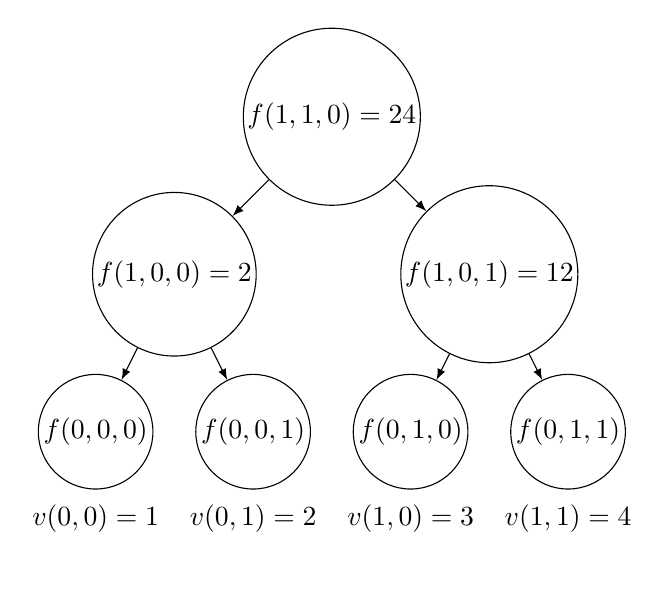
\begin{tikzpicture}[
            level 1/.style={level distance=2cm, sibling distance=4cm},
            level 2/.style={level distance=2cm, sibling distance=2cm},
            level 3/.style={level distance=1.1cm, sibling distance=2cm, edge from parent/.style={draw=none},},
            edge from parent/.style={draw, -latex},
            every node/.style={circle,draw,inner sep=1pt}
        ]
        \node {$f(1,1,0)=24$}
            child {
                node {$f(1,0,0)=2$}
                child { node {$f(0,0,0)$}
                    child { node[draw=none] {$\displaystyle v(0,0)=1$} }
                }
                child { node {$f(0,0,1)$}
                    child { node[draw=none] {$\displaystyle v(0,1)=2$} }
                }
            }
            child {
                node {$f(1,0,1)=12$}
                child { node {$f(0,1,0)$}
                    child { node[draw=none] {$\displaystyle v(1,0)=3$} }
                }
                child { node {$f(0,1,1)$}
                    child { node[draw=none] {$\displaystyle v(1,1)=4$} }
                }
            };
        \end{tikzpicture}
        }

        \vspace{-1em}
        \textit{\textbf{Illustration:} Binary tree of the Grand Product constraints for $v(x_1, x_2) = 1 + 2x_1 + x_2$.}
    \end{center}
\end{example}

Then, to check that $\forall x \in \{0,1\}^{\log m}$ the equation $f(1,x) = f(x, 0) \cdot f(x, 1)$ holds, we can use 
a sum-check protocol to prove the evaluation of $g$ that is referred to a MLE of $f(1,x) - f(x, 0) \cdot f(x, 1)$:
\begin{equation*}
    g(t) = \sum_{x \in \{0,1\}^{\log m}} \widetilde{\text{eq}}(t,x) \cdot (f(1,x) - f(x, 0) \cdot f(x, 1))
\end{equation*}
By the Schwartz–Zippel lemma, except for a soundness error of $\frac{\log m}{|\mathbb{F}|}$ (which should be negligible),
 $g(\tau) = 0$ for $\tau$ uniformly random in $\mathbb{F}^{\log m}$ if and only if $g = 0$, which implies that 
 $f(1, x) - f(x, 0) \cdot f(x, 1) = 0$ for all $x \in \{0, 1\}^{\log m}$.

Similarly, to prove that $v(x) = f(0, x)$ for all $x \in \{0, 1\}^{\log m}$ it suffices to prove that $v(\gamma) = f(0, \gamma)$
 for a public coin $\gamma \in \mathbb{F}^{\log m}$.

Thus, to prove the existence of $f$ and hence the grand product relationship, it suffices
to prove, for some verifier selected random $\tau, \gamma \in \mathbb{F}^\ell$, that:
\begin{gather}
\label{eq:grands0}
    0 = \sum_{x \in \{0,1\}^{\log m}} \widetilde{\text{eq}}(x, \tau) \cdot (f(1,x) - f(x, 0) \cdot f(x, 1))\\
\label{eq:grands1}
    f(0, \gamma) = v(\gamma)\\
\label{eq:grands2}
    f(1,\dots,1, 0) = p
\end{gather}
This can be achieved by running the sum-check protocol between $\mathcal{P}$ and $\mathcal{V}$, where $\mathcal{V}$ 
has oracle access to $v$ and $f$. Additionally, $\mathcal{V}$ evaluates the $f, v$ at the random point $\gamma$ to 
verify that $f(0, x) = v(x)$. So, the sum-check-based protocol for the grand products looks as follows:
\newline
\begin{algorithm}[H]
\caption{Sum-Check-based Protocol for Grand Products}\label{alg:sum_check_grand_product}
\DontPrintSemicolon
\SetAlgoLined

\textbf{$\mathcal P$:}
Compute polynomials 
$v\in\mathbb{F}^{\log m}[x]$, 
$f\in\mathbb{F}^{\log m+1}[x]$ 
such that
\vspace{-0.8em}
\begin{equation*}
    \vspace{-1.6em}
    p = \prod_{x\in\{0,1\}^{\log m}} v(x)
    \quad\text{and}\quad
    f, v \text{ satisfy }(\ref{eq:grands0}),\,(\ref{eq:grands1}),\,(\ref{eq:grands2}).
\end{equation*}\;

\textbf{$\mathcal P$:}
$C_f \leftarrow \textsc{Commit}(f)$;
$C_v \leftarrow \textsc{Commit}(v)$;
send $C_f, C_v$ to $\mathcal V$.\;

\textbf{$\mathcal V$:}
Choose random $\tau,\gamma\in\mathbb{F}^{\log m}$ and send them to $\mathcal P$.\;

\textbf{$\mathcal P$:}
Compute
\vspace{-0.8em}
\begin{equation*}
    \vspace{-1.6em}
    g(x)\;=\;\widetilde{\mathrm{eq}}(x,\tau)\,\bigl(f(1,x)-f(x,0)\,f(x,1)\bigr).
\end{equation*}\;

\textbf{$\mathcal P$ \& $\mathcal V$:}
Run \textsc{SumCheckProtocol}($0,\;g,\;C_f$)

\Comment{we assume this sum‐check runs over the commitment to $f$, not directly on $g$.}

\textbf{$\mathcal V$:}
$r \leftarrow \textsc{Query}(C_f,(1,\dots,1,0))$.\;
\If{$r \neq p$}{
    \textbf{$\mathcal V$ rejects}.\;
}

\textbf{$\mathcal V$:}
$a \leftarrow \textsc{Query}(C_f,(0,\gamma)), \;$ $v(\gamma)\leftarrow \textsc{Query}(C_v,\gamma)$.\;
\If{$a \neq v(\gamma)$}{
    \textbf{$\mathcal V$ rejects}.\;
}
\end{algorithm}

\begin{remark}
    Note, that during the call to the sum-check protocol, we pass the polynomial $g$ in a couple with the 
    commitment to $f$. Here we assume that each invocation of the \textsc{Query} method to $g$ inside the 
    sum-check instance will be more complex: \textbf{instead of evaluating a single function and returning 
    result, we evaluate $f$ at three different points, check the proofs and return results according to the
    construction of $g$}.
\end{remark}

\subsection{Randomized Permutation Check}
\label{sec:randomized-permutation-check}

The goal of the randomized permutation check is to verify, with high probability, whether two length-$n$
vectors over a field $\mathbb{F}$ contain the same multiset of entries (i.e. one is a permutation of the
other), without performing a full sort or pairwise comparison.

\begin{definition}[Reed-Solomon Fingerprinting]
    Let $\mathbf{a} \in \mathbb{F}^{n}$, then for a random $\gamma \in \mathbb{F}$, the Reed-Solomon 
    fingerprinting of $\mathbf{a}$ is defined as:
    \begin{equation*}
        h_{\gamma}(\mathbf{a}) = \sum_{i=0}^{n-1} a_i \cdot \gamma^i.
    \end{equation*}

    $h_{\gamma}(\mathbf{a})$ uniquely identifies the sequence $\mathbf{a}$ with high probability,
    i.e., if $\mathbf{a} \neq \mathbf{b}$, then, according to the Schwartz-Zippel lemma:
    \begin{equation*}
        \Pr[h_{\gamma}(\mathbf{a}) = h_{\gamma}(\mathbf{b})] \leq \frac{n}{|\mathbb{F}|}.
    \end{equation*}
\end{definition}

\begin{definition}[Randomized Permutation Check]
    Let $A$ and $B$ be two multisets of tuples in $\mathbb{F}^n$. Define
    \begin{equation*}
    \mathcal{H}_{\tau,\gamma}(X)\;=\;\prod_{x \in X}\bigl(h_{\gamma}(x)-\tau\bigr).
    \end{equation*}
    Then comparing $\mathcal{H}_{\tau,\gamma}(A)$ and $\mathcal{H}_{\tau,\gamma}(B)$ yields a
    randomized test for whether $A$ and $B$ are permutations of one another. Concretely:
    1. If $A=B$ (as multisets), then  
    \begin{equation*}
        \mathcal{H}_{\tau,\gamma}(A)=\mathcal{H}_{\tau,\gamma}(B)
    \end{equation*}
    with probability 1 over uniform $\tau,\gamma\in\mathbb{F}$.
    2. If $A\neq B$, then
    \begin{equation*}
    \Pr\left[\,\mathcal{H}_{\tau,\gamma}(A)=\mathcal{H}_{\tau,\gamma}(B)\right]\;\le\; \frac{\max(|A|,|B|)}{|\mathbb{F}|}.
    \end{equation*}
\end{definition}

In other words, by first “hashing” each tuple via the map function $h_{\gamma}$ and then taking the 
$\tau$‐shifted product, one obtains a fingerprint that is invariant under permutation but unlikely 
to collide on distinct sets.

\begin{example}
    Consider all operations in $\mathbb{F}_7$, and set $n=3$, $\tau=5$, and $\gamma=3$.  
    Let
    \begin{equation*}
      A = \{(1,2,3),\,(4,0,6)\}, \quad
      B = \{(4,0,6),\,(1,2,3)\},
    \end{equation*}
    First compute the Reed–Solomon fingerprints modulo 7:
    \begin{equation*}
      h_{\gamma}(1,2,3) =1\cdot3^0 + 2\cdot3^1 + 3\cdot3^2 =1 + 6 + 6 =13 \equiv 6,
    \end{equation*}
    \begin{equation*}
      h_{\gamma}(4,0,6) =4\cdot1 + 0\cdot3 + 6\cdot2 =4 + 0 + 12 =16 \equiv 2,
    \end{equation*}
    Now form the shifted products:
    \begin{equation*}
      \mathcal{H}_{\tau,\gamma}(A) =(6-\tau)\,(2-\tau) =(6-5)\,(2-5) =1\cdot(-3)\equiv4,
    \end{equation*}
    \begin{equation*}
      \mathcal{H}_{\tau,\gamma}(B) =(2-5)\,(6-5) =(-3)\cdot1\equiv4,
    \end{equation*}
    so the test \emph{accepts} $A$ vs.\ $B$ (they are indeed permutations). \\

    Now consider a non-permutation $B'$:
    \begin{equation*}
      B' = \{(1,2,3),\,(2,1,3)\}.
    \end{equation*}
    \begin{equation*}
      h_{\gamma}(2,1,3) =2\cdot1 + 1\cdot3 + 3\cdot2 =2 + 3 + 6 =11 \equiv 4.
    \end{equation*}
    \begin{equation*}
      \mathcal{H}_{\tau,\gamma}(B') =(6-5)\,(4-5) =1\cdot(-1)\equiv6\neq4,
    \end{equation*}
    so the test \emph{rejects} $A$ vs.\ $B'$.  
    In this way a single choice of $(\gamma,\tau)$ distinguishes permutations from non-permutations.
\end{example}

\subsection{Offline Read-Only Memory Checking}
\label{sec:offline-memory-checking}

This protocol lets you, after doing a bunch of reads from an untrusted read-only memory, verify in one quick
algebraic step that every answer really came from the same original contents -- without re-running any reads.

For the first time it's not so obvious, why we may need need such a protocol, so let's start with a simple 
example.
\begin{example}
    TODO
\end{example}

\begin{remark}
    As we are talking about a read-only memory, we assume that the write operations happen only once,
    during the initialization phase, and the memory is immutable afterwards.
\end{remark}

In the present version of this protocol, each operation is followed by an increment of the corresponding memory
cell counter (unlike the original version, where the counter was global), it also utilizes only reads, pairing
them with ``synthetic'' writes, and requires only three sets of tuples to work with:
\begin{itemize}
    \item $\mathsf{WS}$ -- contains tuples that represent write operations: $\mathsf{(addr, val, counter_{addr})}$,
    where $\mathsf{val}$ is the value stored at the memory address $\mathsf{addr}$ after the specified counter;
    \item $\mathsf{RS}$ -- contains tuples that represent read operations: $\mathsf{(addr, val, counter_{addr})}$,
    where $\mathsf{val}$ is the value read from the memory address $\mathsf{addr}$ at the specified counter;
    \item $\mathsf{S}$ -- contains tuples such that $\mathsf{WS} = \mathsf{RS} \cup \mathsf{S}$ if and only if 
    all operations were executed correctly; otherwise, no such $\mathsf{S}$ exists that satisfies this equality.
\end{itemize}

You can think of a memory as a vector of values, and a counter as a memory cell timestamp, separately for read
and write operations. At the beginning, $\mathsf{WS}$ is populated with the initial memory state, where all 
counters are set to $0$, indicating that the values were first accessed during the initialization phase, while
the $\mathsf{RS}, \mathsf{S}$ are empty. Then, for each read operation, the untrusted memory is queried at 
$\mathsf{addr}$, returning a pair $\mathsf{(val, counter)}$. The tuple $\mathsf{(addr, val, counter)}$ is 
written in $\mathsf{RS}$, and a corresponding write operation $\mathsf{(addr, val, counter + 1)}$ is added to
$\mathsf{WS}$. After all the read operations are done, one can notice that $\mathsf{S}$ equals the final memory
state. The equality of multisets $\mathsf{WS}$ and $\mathsf{RS} \cup \mathsf{S}$ can be verified by a single 
grand-product check.

Thus, $\mathsf{WS} = \mathsf{RS} \cup \mathsf{S}$ can be written as:
\begin{small}
\begin{align*}
    \mathcal{H}_{\tau,\gamma}(\mathsf{WS})
    &= \mathcal{H}_{\tau,\gamma}(\mathsf{RS})
    \;\cdot\; \mathcal{H}_{\tau,\gamma}(\mathsf{S}),\\
    \prod_{(a,v,t)\in \mathsf{WS}}\bigl(h_{\gamma}(a,v,t)-\tau\bigr)
    &= \prod_{(a,v,t)\in \mathsf{RS}}\bigl(h_{\gamma}(a,v,t)-\tau\bigr)\\
    &\quad\;\cdot\;\prod_{(a,v,t)\in \mathsf{S}}\bigl(h_{\gamma}(a,v,t)-\tau\bigr),\\
    \prod_{(a,v,t)\in \mathsf{WS}}\bigl((a\gamma^2+v\gamma+t)-\tau\bigr)
    &= \prod_{(a,v,t)\in \mathsf{RS}}\bigl((a\gamma^2+v\gamma+t)-\tau\bigr)\\
    &\quad\;\cdot\;\prod_{(a,v,t)\in \mathsf{S}}\bigl((a\gamma^2+v\gamma+t)-\tau\bigr).
\end{align*}
\end{small}

\begin{example}
{
\large
\noindent\textbf{$N^{1/c}=4,\;m=3$}
}

\noindent We track a single \emph{row‑memory}. The algorithm performs three reads.
\begin{center}
    \centering
    \begin{tabular}{|c|c|c|c|c|}
        \hline
        Address & 0 & 1 & 2 & 3 \\ \hline
        Value   & 2 & 5 & 7 & 9 \\ \hline
    \end{tabular}
\end{center}

\medskip
\noindent\textbf{Initial memory (counter $0$):}
\begin{equation*}
\mathsf{WS}_{\text{init}} =\{(0,2,0), \; (1,5,0), \; (2,7,0), \; (3,9,0)\},
\end{equation*}
while 
\begin{equation*}
    \mathsf{RS} = \varnothing \quad \text{and} \quad \mathsf{S} = \varnothing.
\end{equation*}

\medskip
\noindent\textbf{Trace 1 – consistent execution}
\begin{center}
    \begin{tabular}{c|c|c|c}
    \textbf{step} & \textbf{operation} & $\Delta\mathsf{RS}_{\text{step}}$ & $\Delta\mathsf{WS}_{\text{step}}$\\\hline
    1 & read(1)$ \; \to \; (5, 0)$ & $(1,5,0)$ & $(1,5,1)$\\
    2 & read(0)$ \; \to \; (2, 0)$ & $(0,2,0)$ & $(0,2,1)$\\
    3 & read(2)$ \; \to \; (7, 0)$ & $(2,7,0)$ & $(2,7,1)$
    \end{tabular}
\end{center}
After the three steps
\begin{equation*}
    \begin{aligned}
        \mathsf{RS} &= \{(1,5,0), \; (0,2,0), \; (2,7,0)\},\\
        \mathsf{WS} &= \mathsf{WS}_{\text{init}} \cup \{(1,5,1), \; (0,2,1), \; (2,7,1)\}.
    \end{aligned}
\end{equation*}
And we can fill $\mathsf{S}$ with
\begin{equation*}
        \mathsf{S} = \{(0,2,1), \; (1,5,1), \; (2,7,1), \; (3,9,0)\}
\end{equation*}
One can clearly see that $\mathsf{WS} = \mathsf{RS} \cup \mathsf{S}$.
\begin{alignat*}{2}
\mathcal H_{\tau,\gamma}(\mathsf{WS})
  &\;=\; \mathcal H_{\tau,\gamma}(\mathsf{RS})
  &\;\times\;
  &\mathcal H_{\tau,\gamma}(\mathsf{S})
\\
  &\;=\;
    \substack{
      (1\gamma^2+5\gamma+0-\tau)\,(0\gamma^2+2\gamma+0-\tau)\\
      (2\gamma^2+7\gamma+0-\tau)
    }
  &\;\times\;&
    \substack{
      (0\gamma^2+2\gamma+1-\tau)\,(1\gamma^2+5\gamma+1-\tau)\\
      (2\gamma^2+7\gamma+1-\tau)\,(3\gamma^2+9\gamma+0-\tau)
    }.
\end{alignat*}

\medskip
\noindent\textbf{Trace 2 – inconsistent execution}\\
Let the second reading return a wrong value -- $a$, instead of $2$. So, the new trace would look like:
\begin{center}
    \begin{tabular}{c|c|c|c}
    \textbf{step} & \textbf{operation} & $\Delta\mathsf{RS}_{\text{step}}$ & $\Delta\mathsf{WS}_{\text{step}}$\\\hline
    1 & read(1)$ \; \to \; (5, 0)$ & $(1,5,0)$ & $(1,5,1)$\\
    2 & read(0)$ \; \to \; (a, 0)$ & $(0,a,0)$ & $(0,a,1)$\\
    3 & read(2)$ \; \to \; (7, 0)$ & $(2,7,0)$ & $(2,7,1)$
    \end{tabular}
\end{center}
After the three steps
\begin{equation*}
    \begin{aligned}
        \mathsf{RS} &= \{(1,5,0), \; (0,a,0), \; (2,7,0)\},\\
        \mathsf{WS} &= \mathsf{WS}_{\text{init}} \cup \{(1,5,1), \; (0,a,1), \; (2,7,1)\},\\
        \mathsf{S} &\rightarrow\text{ does not exist} 
    \end{aligned}
\end{equation*}
Now, $\mathsf{RS}$ contains $(0, \; a, \; 0)$ while $\mathsf{WS}$ still contains the untouched initial 
tuple $(0, \; 2, \; 0)$. No multiset $\mathsf{S}$ that depends on the valid values and addresses can 
reconcile them, and the verifier \emph{rejects}.
\end{example}

\end{document}


